%=====================================================================
\section{Linear analysis and LQR controllers}\label{sec:linear}
%=====================================================================
\subsection{Controllability: can three rotors steer the failed drone?}
\paragraph{Method.} For both linear models we computed three things (experiment E2, \texttt{analysis.py}):
\begin{enumerate}
  \item The rank of the controllability matrix $\mathcal C = [B, AB, \dots, A^{n-1}B]$. Its columns differ in size by many orders of magnitude (each multiplication by $A$ scales them by about 20), which can make a numerical rank test unreliable. We therefore divide every column by its length before computing the singular values (``scaled rank'').
  \item The PBH test for every eigenvalue $\lambda$ of $A$: the smallest singular value of $[\lambda I - A,\; \tilde B]$, where $\tilde B$ is $B$ rescaled to the size of $A$. A value near zero would mark an uncontrollable mode.
  \item The controllability Gramian over 1\,s, $W_c(T) = \int_0^T e^{As}BB^\top e^{A^\top s}ds$. It is computed exactly with Van Loan's method: the matrix exponential of the block matrix $\begin{psmallmatrix}-A & BB^\top\\ 0 & A^\top\end{psmallmatrix}T$ contains $W_c$ in its blocks. This works even for the undamped modes, where the infinite-time Gramian does not exist.
\end{enumerate}

\paragraph{Result.} Both models are controllable. The failed model has rank 7 of 7, and every mode passes the PBH test (smallest values between 0.016 and 0.28, none near zero). The Gramian's smallest eigenvalue is 0.54 and its condition number $7.6\times10^3$: some directions need much more effort than others, but none is out of reach. This reproduces the paper's controllability result; it is not a new finding.

\subsection{Observability: what can the sensors see?}
\paragraph{Method.} A controller needs the state, so we asked which sensors make it observable. For each sensor set we built the output matrix $C$, checked the rank of the observability matrix, and computed the 1\,s observability Gramian. Different sensors measure different units with different noise, so before computing the Gramian we divided each output by an assumed noise level (one standard deviation): gyroscope 0.005\,rad/s, position 0.01\,m, attitude 0.01\,rad, magnetometer heading 0.02\,rad, tilt estimate 0.01, barometer 0.1\,m. The Gramian is then dimensionless, and its smallest eigenvalue says how well the weakest direction is seen \emph{relative to the noise}.

\begin{table}[h]
\centering\small
\caption{Observability of the failed drone's linear model (7 states) for four sensor sets.}\label{tab:obs}
\begin{tabular}{lccc}
\toprule
Sensors & Rank & Cannot see & Smallest eigenvalue of $W_o(1\,\mathrm{s})$ \\
\midrule
Gyroscope $(p,q,r)$ & 3/7 & $n_x, n_y, z, v_z$ & 0 \\
Gyroscope + tilt estimate $(n_x, n_y)$ & 5/7 & $z, v_z$ & 0 \\
Gyroscope + barometer $(z)$ & 7/7 & nothing & $2.4\times10^{-3}$ \\
Gyroscope + tilt + barometer & 7/7 & nothing & 6.6 \\
\bottomrule
\end{tabular}
\end{table}

\paragraph{Reading.} Gyroscopes measure rotation rates only. Because the rate equations do not depend on $\vect n$ (the first three rows of $A$ have zeros in the $\vect n$ columns), the rates carry no information about the tilt, so gyroscopes alone see neither tilt nor height. A small finding of ours: because the relaxed hover is \emph{tilted}, the vertical acceleration depends on the tilt to first order ($A_{v_z n_y} = -2.91$), so a barometer that measures height also reveals the tilt, and gyroscope plus barometer is enough in principle. With realistic noise, however, the smallest eigenvalue of the noise-normalized Gramian is $2.4\times10^{-3}$, against 6.6 with a direct tilt measurement: about 2,700 times smaller, which corresponds to roughly 50 times larger estimation error (standard deviation) in the weakest direction. It is a structural remark, not a practical estimator; real estimators for the spinning drone use inertial sensors together with vision~\cite{sun2021vision} or a magnetometer~\cite{solanki2022attitude}. For the healthy drone, gyroscope plus position leaves the heading unobservable (heading enters the motion only at second order near hover), as expected, and a magnetometer fixes it.

\subsection{LQR controllers}
\paragraph{Healthy LQR.} On the 12-state hover model we used Bryson's rule with largest acceptable errors 0.5\,m horizontal and 0.3\,m vertical position, 1\,m/s horizontal and 0.5\,m/s vertical speed, 0.2\,rad roll and pitch, 0.5\,rad yaw, 2\,rad/s body rates, and 0.5\,N per rotor. A factor $\alpha$ multiplies all state weights, to make the controller more ($\alpha>1$) or less ($\alpha<1$) aggressive. The controller converts the quaternion to Euler angles, wraps the yaw error to $[-\pi,\pi]$, and clips the commands to $[f_{\min}, f_{\max}]$.

\paragraph{Failure LQR.} On the 10-state model (7 states and 3 motor states) we used the paper's weights: 1 on $p$ and $q$, 20 on $n_x$ and $n_y$, 0 on the motor states, and 1\,N$^{-2}$ on each input. The paper's reduced state does not contain $r$; we include it with weight 0 (our choice), and we added 4 on height and 1 on vertical speed, because we also control altitude. The control law is
\begin{equation}
  \vect u = \bar{\vect f} - K\,\big(\vect s - \bar{\vect s},\; \hat{\vect f} - \bar{\vect f}\big), \qquad \text{clipped to } [f_{\min}, f_{\max}],
\end{equation}
where $\hat{\vect f}$ is an estimate of the motor thrusts. Motor thrusts are not measured, so the controller reconstructs them by passing its own commands through the same first-order lag: $\hat{\vect f}_{k+1} = \hat{\vect f}_k + (1-e^{-\Delta t/\sigma})(\vect u_k - \hat{\vect f}_k)$. When the controller is switched on after a failure, this estimate is initialized from what the flight computer knows (a filter of the commands sent before), not from the true thrust, which it cannot measure.

\begin{codebox}{the failure LQR}
\begin{lstlisting}
def __call__(self, t, x):
    s = self.state7(x)                       # (p, q, r, n_x, n_y, z, v_z) from the 17-state
    e = s - self.base.x_trim                 # deviation from the relaxed hover
    e[5] -= self.z_ref
    e = np.concatenate((e, self.f_est - self.eq.f[:3]))     # add motor-state estimate
    u3 = np.clip(self.eq.f[:3] - self.K @ e, self.p.f_min, self.p.f_max)
    self.f_est += (1 - np.exp(-dt / self.p.sigma_mot)) * (u3 - self.f_est)   # exact lag step
    return np.array([u3[0], u3[1], u3[2], 0.0])          # rotor 4 gets nothing
\end{lstlisting}
\end{codebox}

\paragraph{Delay margin.} To find how much pure input delay $h$ each loop tolerates, we discretize the linear loop exactly at 1\,ms and append a chain of $h/1\,\text{ms}$ memory states that pass the command along (a ``delay line''). The loop is stable if all eigenvalues of this larger matrix lie inside the unit circle. We increase $h$ in 1\,ms steps from zero and stop at the first unstable value.

\begin{table}[h]
\centering\small
\caption{LQR designs (experiment E3).}\label{tab:lqr}
\begin{tabular}{lll}
\toprule
Controller & Slowest closed-loop poles & Delay margin \\
\midrule
Healthy LQR (12 states) & $-1.72\pm1.02j$, $-1.89$, $-1.94\pm1.56j$ & 40\,ms \\
Failure LQR (7 + 3 motor states) & $-1.09$, $-2.01\pm1.04j$, $-3.80\pm19.68j$ & 18\,ms \\
Failure LQR without motor states & $-1.09$, $-2.01\pm1.04j$, $-3.83\pm19.66j$ & 18\,ms \\
\bottomrule
\end{tabular}
\end{table}

\paragraph{Results.} All closed-loop poles have negative real parts. The least-damped mode of the failure LQR is the oscillation near the spin frequency, $-3.80\pm19.68j$, with damping ratio about 0.19. The failure LQR tolerates only 18\,ms of input delay, against 40\,ms for the healthy one: the spinning drone is a much less forgiving system. The design without motor states remains stable when the real 15\,ms motor lag is present (largest real part $-1.10$), but we follow the paper and include the motors.

On the full nonlinear model with motor lag and thrust limits, we started the failure LQR at the relaxed hover with rate errors $(1, -1, -3)$\,rad/s, tilt errors $(0.08, -0.05)$ and 1\,m below the set-point (Figure~\ref{fig:lqr}). It returned to the equilibrium: the tilt settled within 0.01 in 2.1\,s, the height within 5\,cm in 1.8\,s and the yaw rate within 0.5\,rad/s in 2.5\,s. After 6\,s the remaining errors were $1.6\times10^{-4}$ in tilt and 0.012\,rad/s in rate. The healthy LQR, started 0.5\,m off and tilted by up to 0.4\,rad, returned to within 0.25\,mm in 5\,s (Figure~\ref{fig:lqr-healthy}).

\begin{figure}[h]
\centering
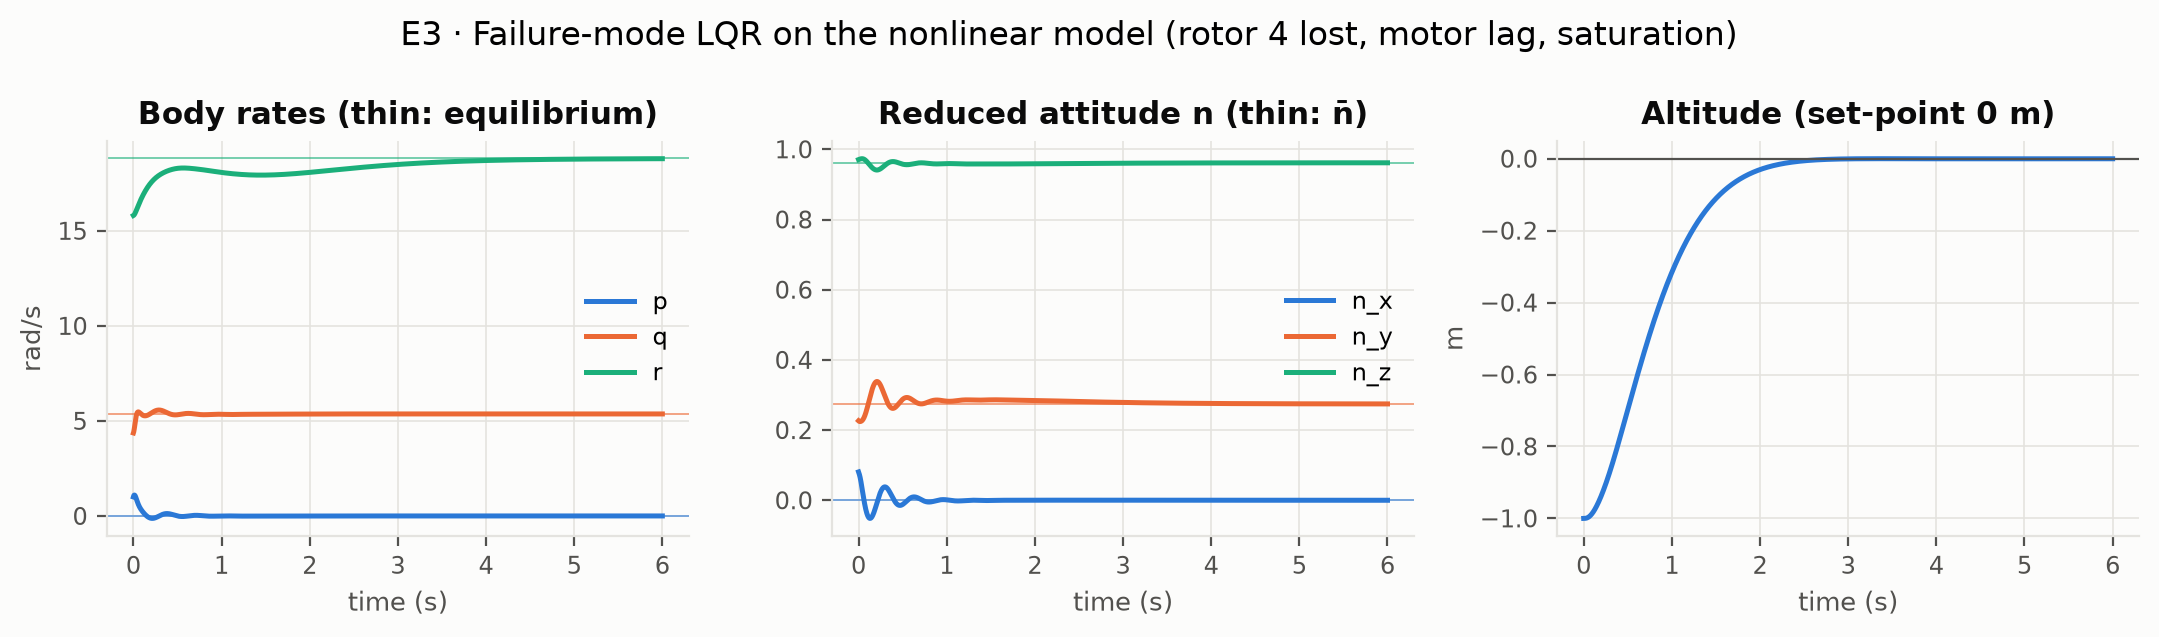
\includegraphics[width=\linewidth]{figures/e3_failed_lqr_nonlinear.png}
\caption{Failure LQR on the nonlinear model (rotor 4 lost, motor lag, thrust limits), starting from a perturbed relaxed hover 1\,m below the set-point. Thin lines: equilibrium values.}\label{fig:lqr}
\end{figure}
\begin{figure}[h]
\centering
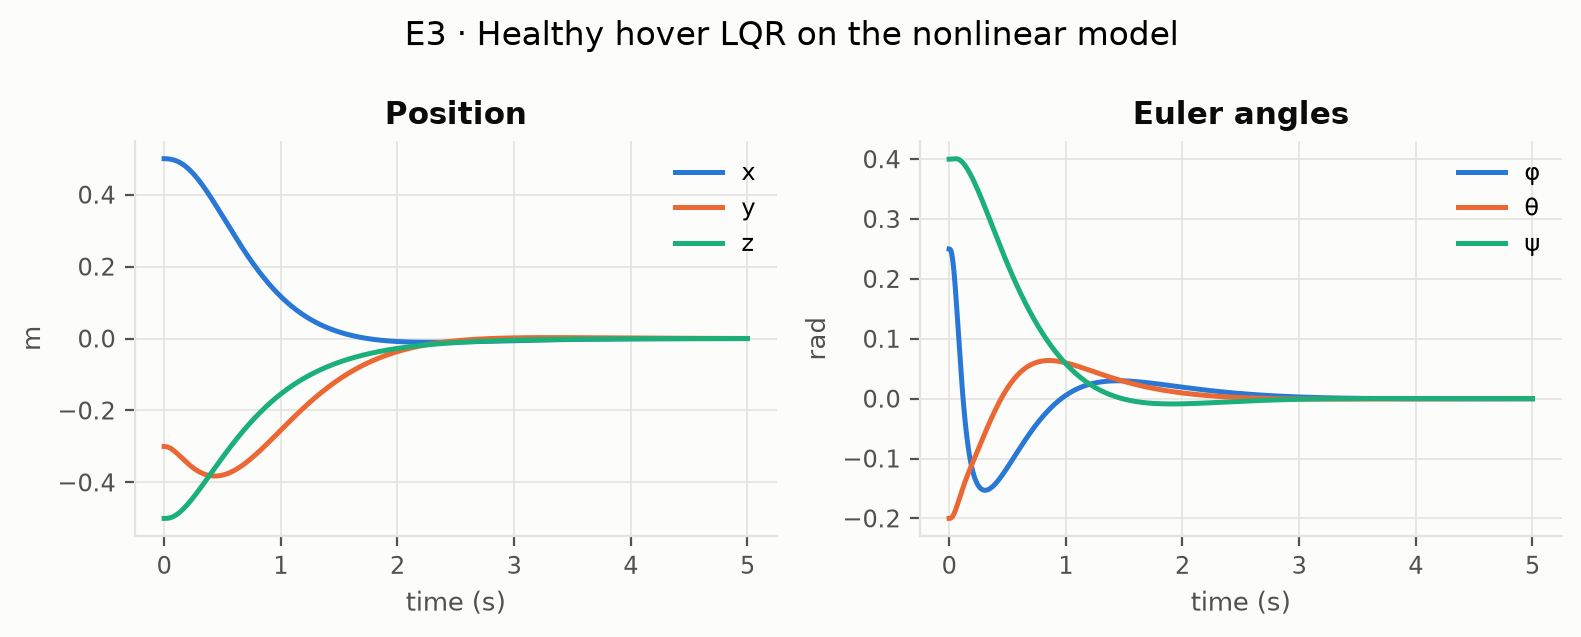
\includegraphics[width=0.75\linewidth]{figures/e3_healthy_lqr_nonlinear.png}
\caption{Healthy LQR on the nonlinear model from an offset, tilted start.}\label{fig:lqr-healthy}
\end{figure}
